\chapter{Case setup}
\section{A test case}
With the help of the OpenFOAM tutorial case study, a test case was set up
for the simulation of multiphase flow over a NACA0012 hydrofoil. The geometry is from a compressible flow tutorial 
where  k-$\omega$ sst turbulence model was adopted. The $\textit{blockMeshDict}$ of tutorial is relevant for the thesis by helping 
to tune the mesh based on requirement. To set up the case folders for multiphase flow, another case study 
tutorial is used: multiphase/interFoam/RAS/propeller. The mass transfer model used in the tutorial is 
Schnerr-Sauer, which relevant for  thesis and also the tutorial assists with setting up 
the 3 folders to run the simulation properly. In the working directory, copy the essential 
files from the tutorials. The case setup of the working directory contains three folders 
$\textit {0/, constant/, and system/}$, with slight modification is made in all three 
of them as outlined below.
\section{Computational domain}
The flow field around the hydrofoil is modeled in three-dimension with negligible 
dimension in span wise direction. 
\begin{figure}[H]
    \centering
    \includegraphics[scale=0.4]{blockMesh.png}
    \caption{Schematic representation of flow field around NACA0012 hydrofoil with boundary condition}
    \label{fig:fig16}
\end{figure}
\subsection{Boundary and initial condition}
The boundary condition and parameters of work condition  are taken from the reference
\cite{Zhao2021} which is stated below:
\begin{table}[h]
    \centering
    \begin{tabular}{|c|c|}
    \hline
        hydrofoil & Wall \\
    \hline
        inlet & Velocity \\ 
    \hline
       outlet & Pressure  \\
    \hline
       top and bottom & Symmetry \\
   \hline
    \end{tabular}
    \caption{Boundary condition}
    \label{tab:BC}
\end{table}
The parameter of working condition is stated below:
\begin{table}[h]
    \centering
    \begin{tabular}{|c|c|}
    \hline
        Velocity(U) & 5 m/s \\
    \hline
        Cavitation number ($\sigma$) & 0.8 \\ 
    \hline
     Turbulence kinetic energy(K) & 0.0185 \\
    \hline
    Specific dissipation rate($\omega$) & 621.626 \\
    \hline
    pressure($P_v$) & 9358.6848 N/${m}^2$\\
    \hline
    Reference pressure($P_{out}$) &  0.203e5 N/${m}^2$ \\
    \hline
    Chord length(C) & 100 mm \\
    \hline
    Angle of attack($\alpha$) & ${3.2}^{\circ}$ to ${8}^{\circ}$ \\
   \hline
    \end{tabular}
    \caption{parameters of work condition}
    \label{tab:PC}
\end{table}
\section{Grid study}
In thesis, the influence of mesh size was discussed. Three types of mesh were analyzed to 
determine the appropriate mesh size for numerical simulation. It was clear that the force coefficient increased when
mesh size was small. It can be seen from the verification and validation results that the value of numerical 
uncertainty is larger than the comparison error. Thus, the calculated results are in agreement, but there 
is not enough evidence to confirm their accuracy.
\begin{table}[h]
\centering
\begin{tabular}{|l|l|l|l|l|l|}
\hline
 Grid no& No of cells & No of faces &No of nodes  & Cl & Cd \\ \hline
 &  &  &  &  &  \\ \hline
 &  &  &  &  &  \\ \hline
 &  &  &  &  &  \\ \hline
\end{tabular}
\caption{}
\label{}
\end{table}
\begin{figure}[H]
    \centering
    \includegraphics[scale=0.4]{gridstudy.png}
    \caption{Grid lines in coarse mesh over view}
    \label{fig:fig17}
\end{figure}
\section{Case folder setup}
\subsection{0 Folder} This folder should be initilized with the working parameters such 
as velocity as ${\textit {U}}/$ which is a reference velocity, ${\textit{p}}_{{\textit {\_rgh}}}/$  
reference pressure, ${\textit {omega}}/$ specific dissipation rate, ${\textit {k}}/$ 
turbulence kinetic energy, ${\textit {nut}}/$, ${\textit {alpha.water}}/$ vapour fraction 
respectively. Inorder to include the angle of attack on the hydrofoil it is better to specify the velocity as 
$V_x$=V$cos \alpha$ and $V_z$=$V sin \alpha$(normal direction is in z direction). The internalField and 
boundaryField of each files in the $0/$folder are stated below:\\ 
\begin{table}[h]
\centering
\begin{tabular}{|ll|ll|lll}
\cline{1-4}
\multicolumn{1}{|l|}{Parameters} & internalField & \multicolumn{2}{l|}{boundaryField}    &  &  &  \\ \cline{1-4}
\multicolumn{2}{|l|}{}    & \multicolumn{1}{l|}{freestream} & wall &  &  &  \\ \cline{1-4}
\multicolumn{1}{|l|}{U} & uniform $\$Uinlet$ & \multicolumn{1}{l|}{ type:            freestreamVelocity} &  type:            noSlip &  &  &  \\ \cline{1-4}
\multicolumn{1}{|l|}{pOut} & uniform $\$pOut$ & \multicolumn{1}{l|}{type:            freestreamPressure} &type:            fixedFluxPressure  &  &  &  \\ \cline{1-4}
\multicolumn{1}{|l|}{omegaInlet} & uniform $\$omegaInlet$ & \multicolumn{1}{l|}{type:            inletOutlet} & type:           omegaWallFunction &  &  &  \\ \cline{1-4}
\multicolumn{1}{|l|}{kInlet} & uniform $\$kInlet$ & \multicolumn{1}{l|}{type:           calculated} & type:            kqRWallFunction  &  &  &  \\ \cline{1-4}
\multicolumn{1}{|l|}{nut} & uniform 0  & \multicolumn{1}{l|}{type:            calculated} & type:            nutkWallFunction &  &  &  \\ \cline{1-4}
\end{tabular}
\caption{Condition of parameters of each files of 0$/$ folder}
 \label{tab:PC}
\end{table}
\begin{table}[h]
\centering
\begin{tabular}{|l|l|lll|}
\hline
Parameter& internalField  & \multicolumn{3}{l|}{boundaryField}                            \\ \hline
&  & \multicolumn{1}{l|}{inlet} & \multicolumn{1}{l|}{outlet} &  wall \\ \hline
alpha.water & uniform 1 & \multicolumn{1}{l|}{type:            fixedValue} & \multicolumn{1}{l|}{type:            inletOutlet} &type:            zeroGradient  \\ \hline
\end{tabular}
\caption{Condition of parameter of alpha.water files of 0$/$ folder}
\label{tab:PC}
\end{table}



In boundaryField, the freestream takes the value as uniform as declared in the internalField. The wall in 
the boundaryField is nothing but hydrofoil and some parameters requires value which is also declared from 
the internalField.

\subsection{Constant folder}
This folders enclosed with 4 files such as $\textit{g}/$, $\textit{momentum transport}/$, 
$\textit{phaseChangeProperties}/$, $\textit{transportProperties}/$. There are also two folders geometry 
and polyMesh. In $\textit{geometry}/$, the folder is enclosed with NACA0012.obj file which helps to run 
$\textit{ \$/blockMesh}$ command in the working directory to generate $\textit{polyMesh}/$ folder in the 
constant folder. This folder carries files such as $\textit{boundary}/$, $\textit{face}/$, $\textit{neighbor}/$, 
$\textit{owner}/$, $\textit{points}/$.\\The $\textit{momentumTransport/}$ file is the place for the declaration 
of turbulence model.
\begin{table}[h]
\centering
\begin{tabular}{|lll|}
\hline
\multicolumn{3}{|l|}{momentumTransport}                            \\ \hline
\multicolumn{1}{|l|}{simulationType } & \multicolumn{1}{l|}{RAS} & model:          kOmegaSST \\ \hline
\end{tabular}
\caption{Parameters in momentumTransport}
\label{tab:PC}
\end{table}








\begin{table}[h]
\centering
\begin{tabular}{|ccc|}
\hline
\multicolumn{3}{|c|}{PhaseChangeProperties}                            \\ \hline
\multicolumn{1}{|c|}{phaseChangeModel} & \multicolumn{1}{c|}{SchnerrSauer} & SchnerrSauerCoeffs on \\ \hline
\multicolumn{1}{|c|}{pSat(saturation vapor pressure)} & \multicolumn{2}{c|}{9358.6848}    \\ \hline
\end{tabular}
\caption{Parameters in phaseChangeProperties}
\label{tab:PC}
\end{table}







\begin{table}[h]
\centering
\begin{tabular}{|ll|}
\hline
\multicolumn{2}{|l|}{transportProperties}    \\ \hline
\multicolumn{1}{|l|}{phases} &water vapour  \\ \hline
\multicolumn{1}{|l|}{pSat} & 9358.6848 \\ \hline
\multicolumn{1}{|l|}{sigma(cavitation number) } & 0.8 \\ \hline
\end{tabular}
\caption{Parameters in transportProperties}
\label{tab:PC}
\end{table}












The $\textit{phaseChangeProperties/}$ file is the place for the declaration of mass transfer model and saturation vapor pressure. The
$\textit{transportProperties}/$ is the place to declare the phase of a mixture, its properties, as well as the cavitation number.
\subsection{System folder}
This folder contains files such as  $\textit{blockMeshDict}/$, $\textit{controlDict}/$, $\textit{decomposeParDict}/$, 
$\textit{extrudeMeshDict}/$, $\textit{fvScheme}/$, $\textit{fvSolution}/$.\\
\subsubsection{Time step control}
The court number affects the reliability and stability of the unstable flow simulation. The maxCo should 
be set around 5 in the $\textit{controlDict}/$ file. Therefore set  detlaT as 1e-5 seconds in system/controDict/. Note that cavitating flow calculations 
should always be initiated from a flow field. When cavitation is toggled on, simulation must be restarted from the 
current flow field.\\
\subsubsection{Discretisation schemes}
In OpenFOAM, the free surface treatment does not account for turbulence. All free surface simulations can be viewed 
as direct numerical simulations (DNS). Therefore there is a high requirement for the mesh resolution of the interface. 
The solver uses the multidimensional universal limiter for explicit solutions (MULES) to maintain the boundedness of 
the phase fraction, regardless of the underlying numerical scheme, mesh structure, etc. The choice of schemes for 
convection is therefore not restricted to those that are strongly stable or bounded, e.g. upwind differencing.\\
\subsubsection{Solution and algorithm control}
The $\textit{system/fvSolution/}$ file controls the equation solvers, tolerance and algorithms. 
In first subdictionary, solver, each linear-solver used for each discretized equation is specified. This is achieved by
specifying the solver of each variable being solved, in this case, which is: pcorr (pressure corrector), p$\_$rgh, p$\_$rghFinal
(the final value of pressure after the correction), $(U|k|omega)$, $(U|k|omega)Final$ and alpha.water. The variable name is followed via the
solver name and a dictionary containing the parameters that the solver uses. The pressure variables are solved with the aid of solver GAMG 
and smoother as DICGaussSeidel(Diagonal Incomplete Cholesky), velocity and turbulence quantities is solved using a solver 
smoothSolver and smoother symGaussSeidel, and volume fraction alpha.water by way of MULES. The tolerance, and ratio of 
current to initial residuals, relTol, are specified afterward. The solver stops if either of the tolerance falls 
beneath the targeted value. The precept of GAMG is to generate a quick solution on a mesh with a small number of cells, 
map this solution onto a finer mesh, use it as an initial guess to obtain an correct solution on the fine mesh.\\
\begin{figure}[H]
    \centering
    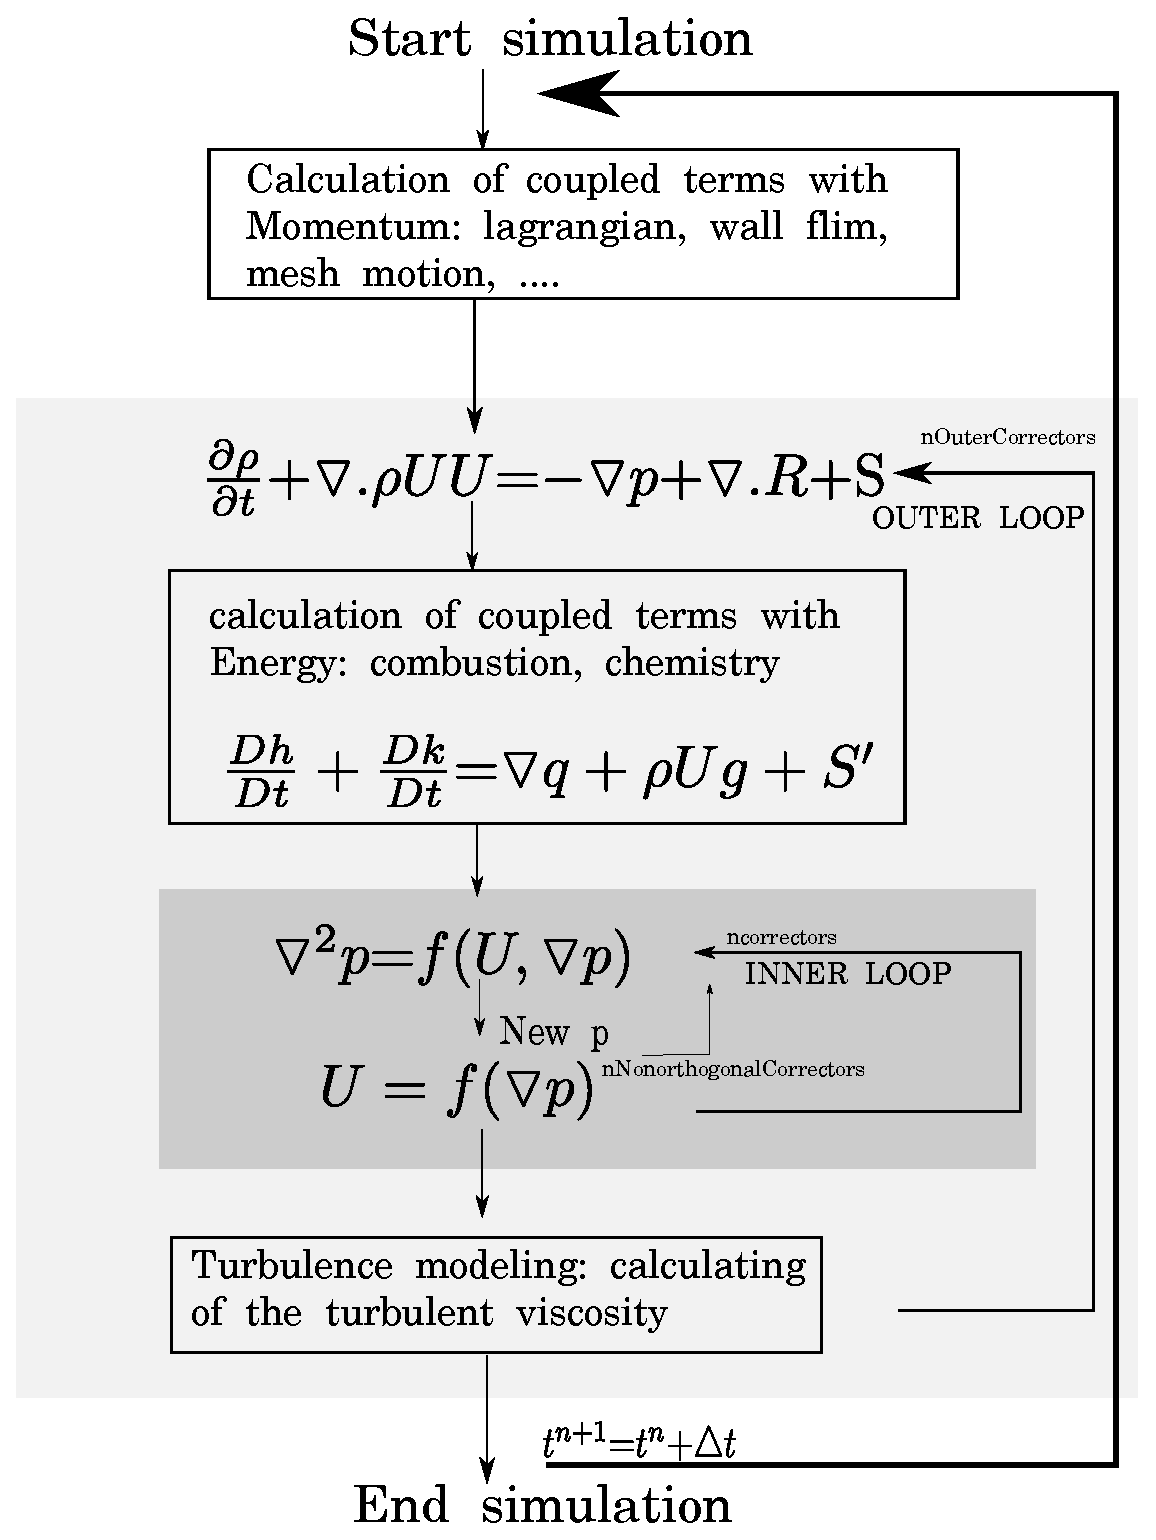
\includegraphics[scale=0.4]{PIMPLEflowchart}
    \caption{rhoPimpleFoam-based solvers}
    \label{fig:fig16}
\end{figure}

In OpenFOAM, any compressible flow solver is usually based on PIMPLE, which is an algorithm of iterative procedures 
for solving equations for velocity and pressure of unsteady problems. PIMPLE is an unsteady, transient SIMPLE.
The number of correctors is specified by the keyword nCorrectors which should be greater than 1. The number of non-orthogonal correctors is specified by the 
nNonOrthogonalCorrectors keyword to account for mesh non-orthogonality which should be greater than 1. An orthogonal mesh is one for which the face normal 
is parallel to the vector between the centers of the adjacent cells, for example, a mesh of hexagonal cells whose faces are 
aligned with a Cartesian coordinate system. In the thesis, nOuterCorrectors should be set to 3, nCorrectors to 1, and nNonOrthogonalCorrectors to 0.
\subsection{Postprocessing}
To validate the force in the x and z direction it is better to use the force function object. This forces function
object generates hydrodynamic force and moment data for surfaces. The forces comprise normal pressure
and tangential viscous contributions. The forces obtained from the postprocessing is used for calculating the
Cl and Cd. The basic operation of the forces function object is cited in controlDict/ which comprises
mandatory entries stated below:\\
\begin{table}[h]
\centering
\begin{tabular}{|ll|}
\hline
\multicolumn{2}{|l|}{forces1}    \\ \hline
\multicolumn{1}{|l|}{type } &forces  \\ \hline
\multicolumn{1}{|l|}{libs} & libforces.so  \\ \hline
\multicolumn{1}{|l|}{patches} & hydrofoil(wall) \\ \hline
\end{tabular}
\caption{Forces function object}
\label{tab:PC}
\end{table}




Inorder to validate the term yplus the yPlus function object is used computes the near wall $y^+$ for turbulence models
by using yPlus functions sub-dictionary in $\textit{system/controlDict}/$. It is better to use ${\#includeFunc}$ $yPlus/$ 
in the function of $\textit{controlDict}/$.
The pressure function object provides to validate the total pressure coefficient. The following  mandatory entries are 
included in the function of $\textit{controlDict}/$ are stated below: 
 \begin{table}[h]
\centering
\begin{tabular}{|ll|}
\hline
\multicolumn{2}{|l|}{pressure1}    \\ \hline
\multicolumn{1}{|l|}{type } &pressure  \\ \hline
\multicolumn{1}{|l|}{libs} & libfieldFunctionObjects.so  \\ \hline
\multicolumn{1}{|l|}{mode} & totalCoeff \\ \hline
\end{tabular}
\caption{Pressure function object}
\label{tab:PC}
\end{table}

















